\section{Target}

The CLAS12 target components are imported from the engineering model. The STEP files are converted to tessellated STL files and imported
in the GEMC simulation \cite{targetCorrection}, \cite{targetStudy}.

An example of the tessellation is shown in \F{targetScatteringChamber}.

\begin{figure}
	\centering
	\includegraphics[width=0.95\columnwidth,keepaspectratio]{img/targetScatteringChamber.png}
	\caption{An example of volume from a STP file tessellated in GEMC. The volume that is shown is the target scattering chamber.
            Top: the CAD representation in the engineering model. Bottom: the tessellation. }
	\label{fig:targetScatteringChamber}
\end{figure}

Key elements of the STL import include the torlon tube to the target cell,
the target aluminum windows and kapton walls and the scattering chamber, see \F{targetDesign}.

\begin{figure}
	\centering
	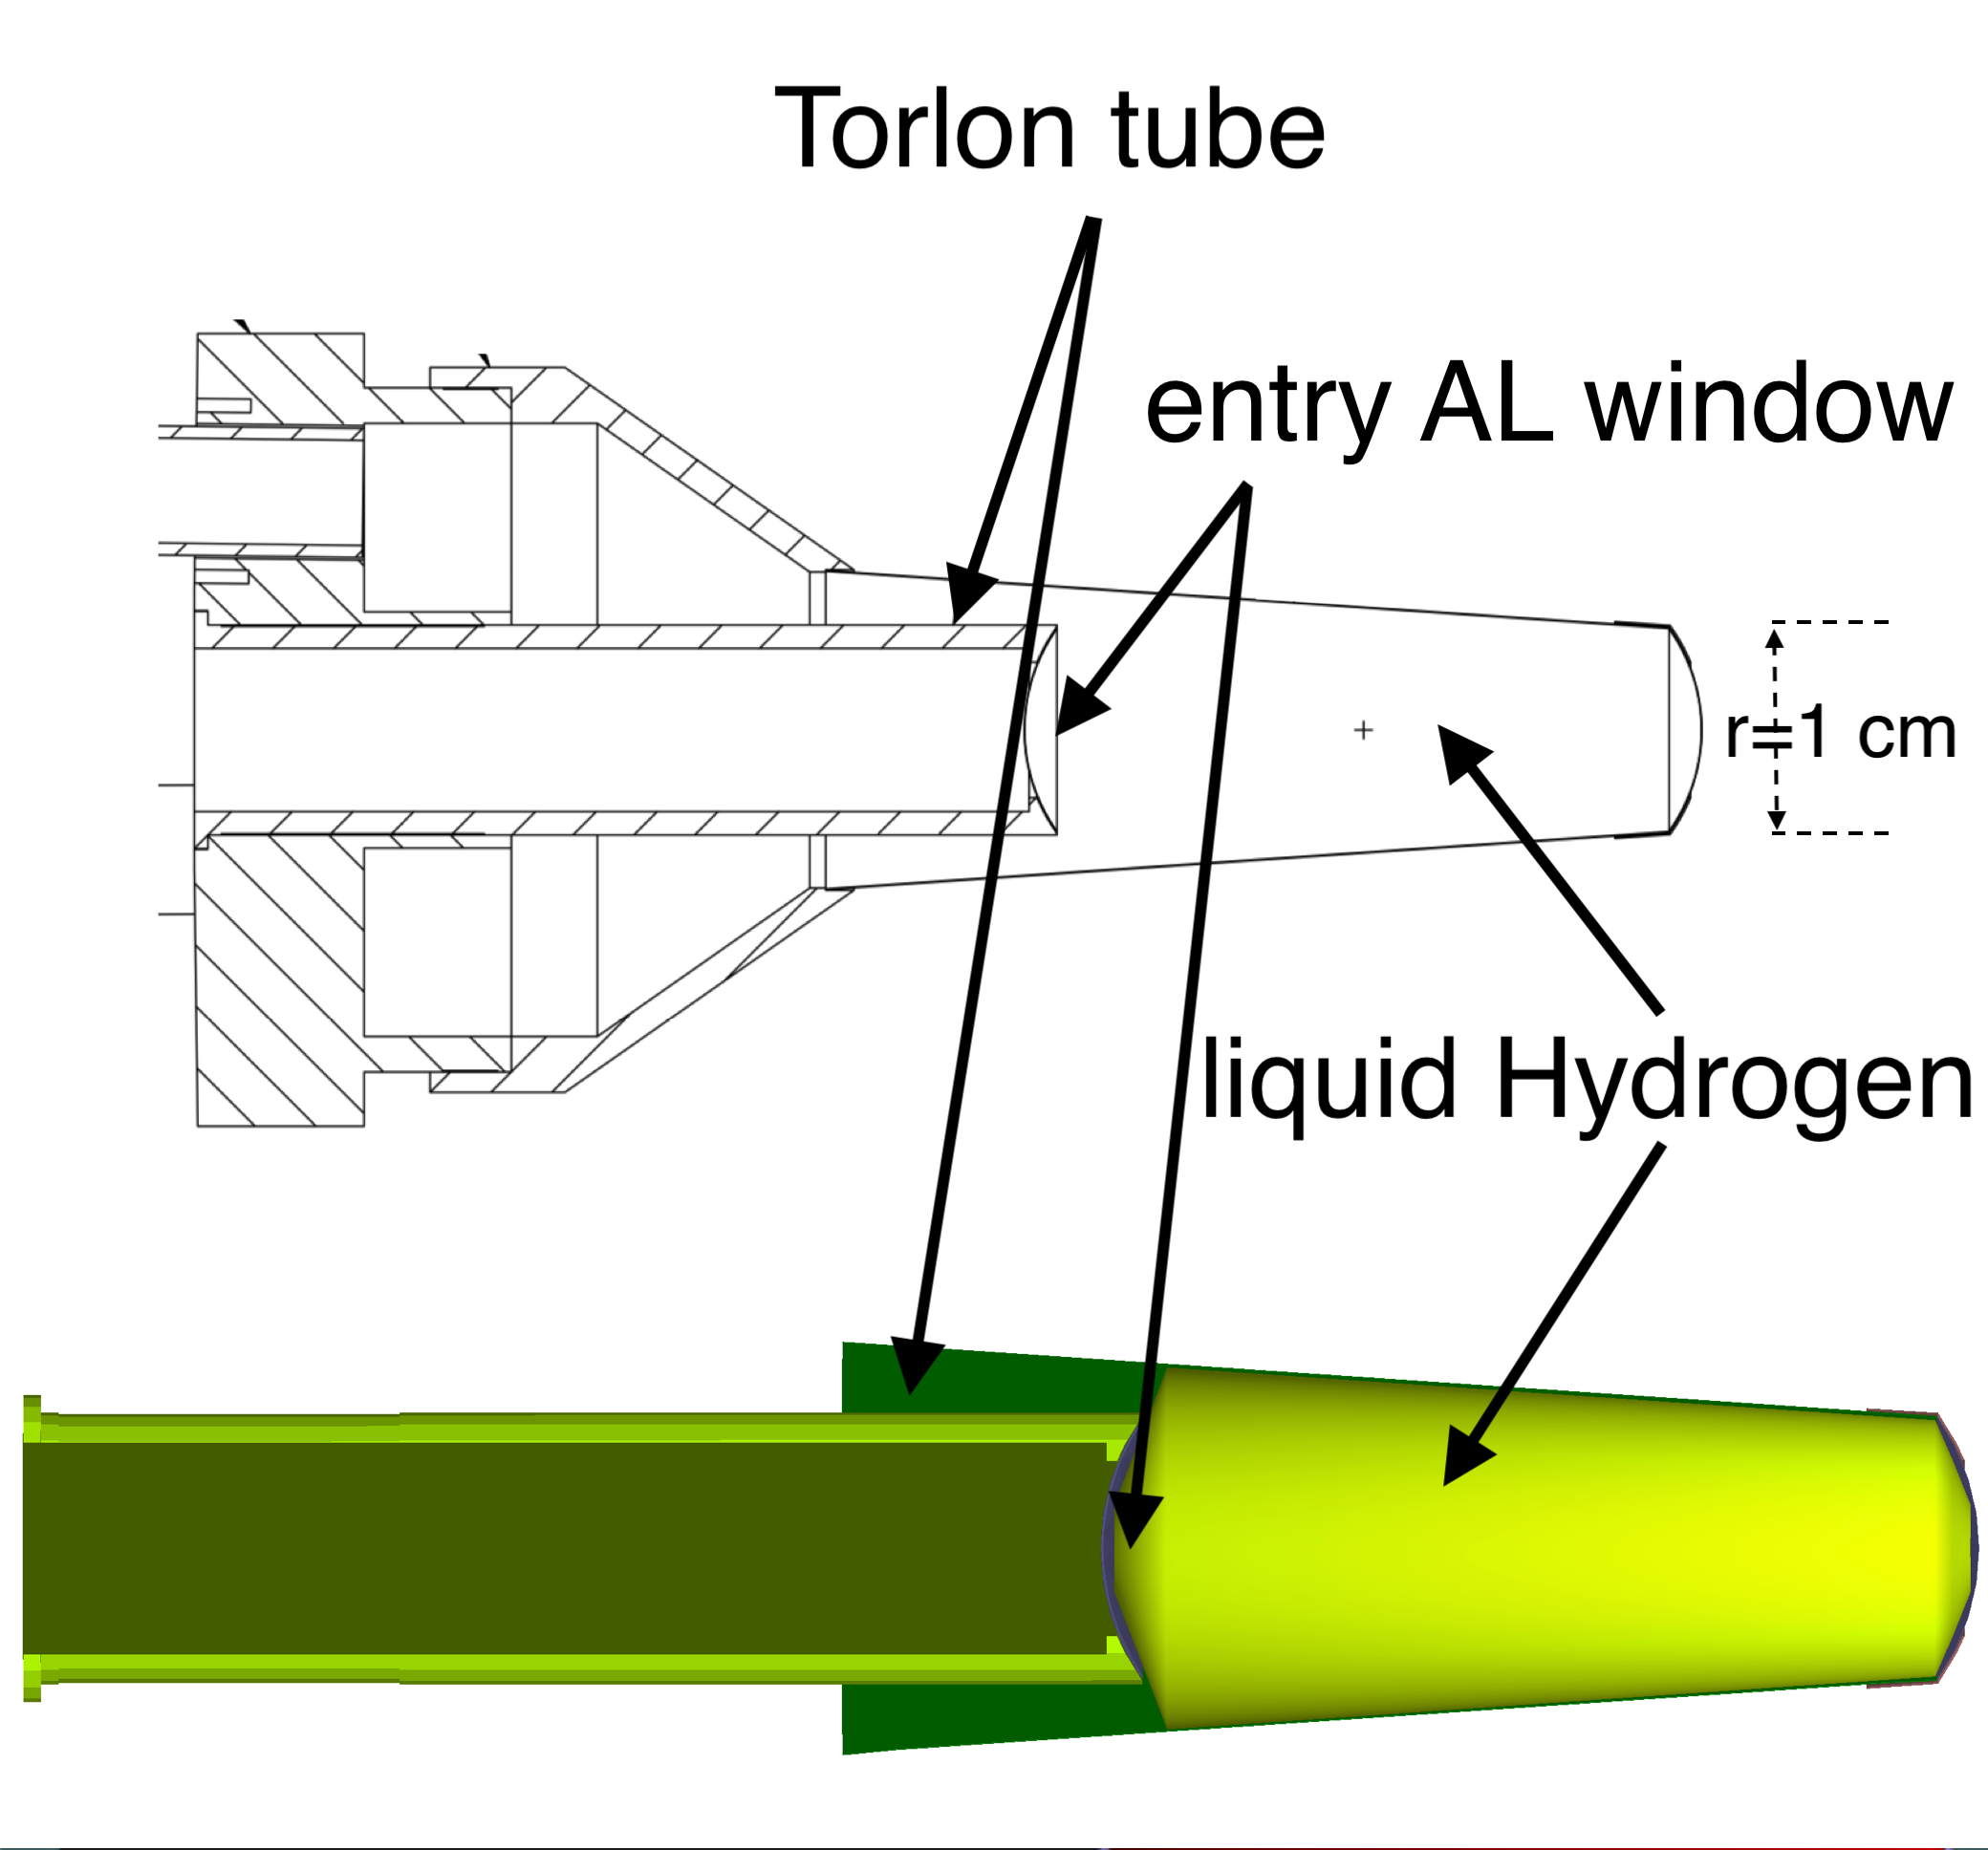
\includegraphics[width=0.95\columnwidth,keepaspectratio]{img/targetDesign.png}
	\caption{The CLAS12 target design. Top left: the entry assembly schematic. Top right: the liquid hydrogen cell
            dimensions: the outer radius is tapered down from 15 mm at z=-2.5cm to 10mm at z=2.5mm.
            Bottom left: The cell implementation in GEMC from the CAD drawings. From left to right (beam direction):
            the black torlon tube, the upstream aluminum window, the target cell, the kapton cup and the
				downstream aluminum window. Bottom right: the GEMC implementation of the kapton cup.}
	\label{fig:targetDesign}
\end{figure}

An overview of the target in geant4 and the engineering model is shown in \F{targetOverview}.

\begin{figure}
	\centering
	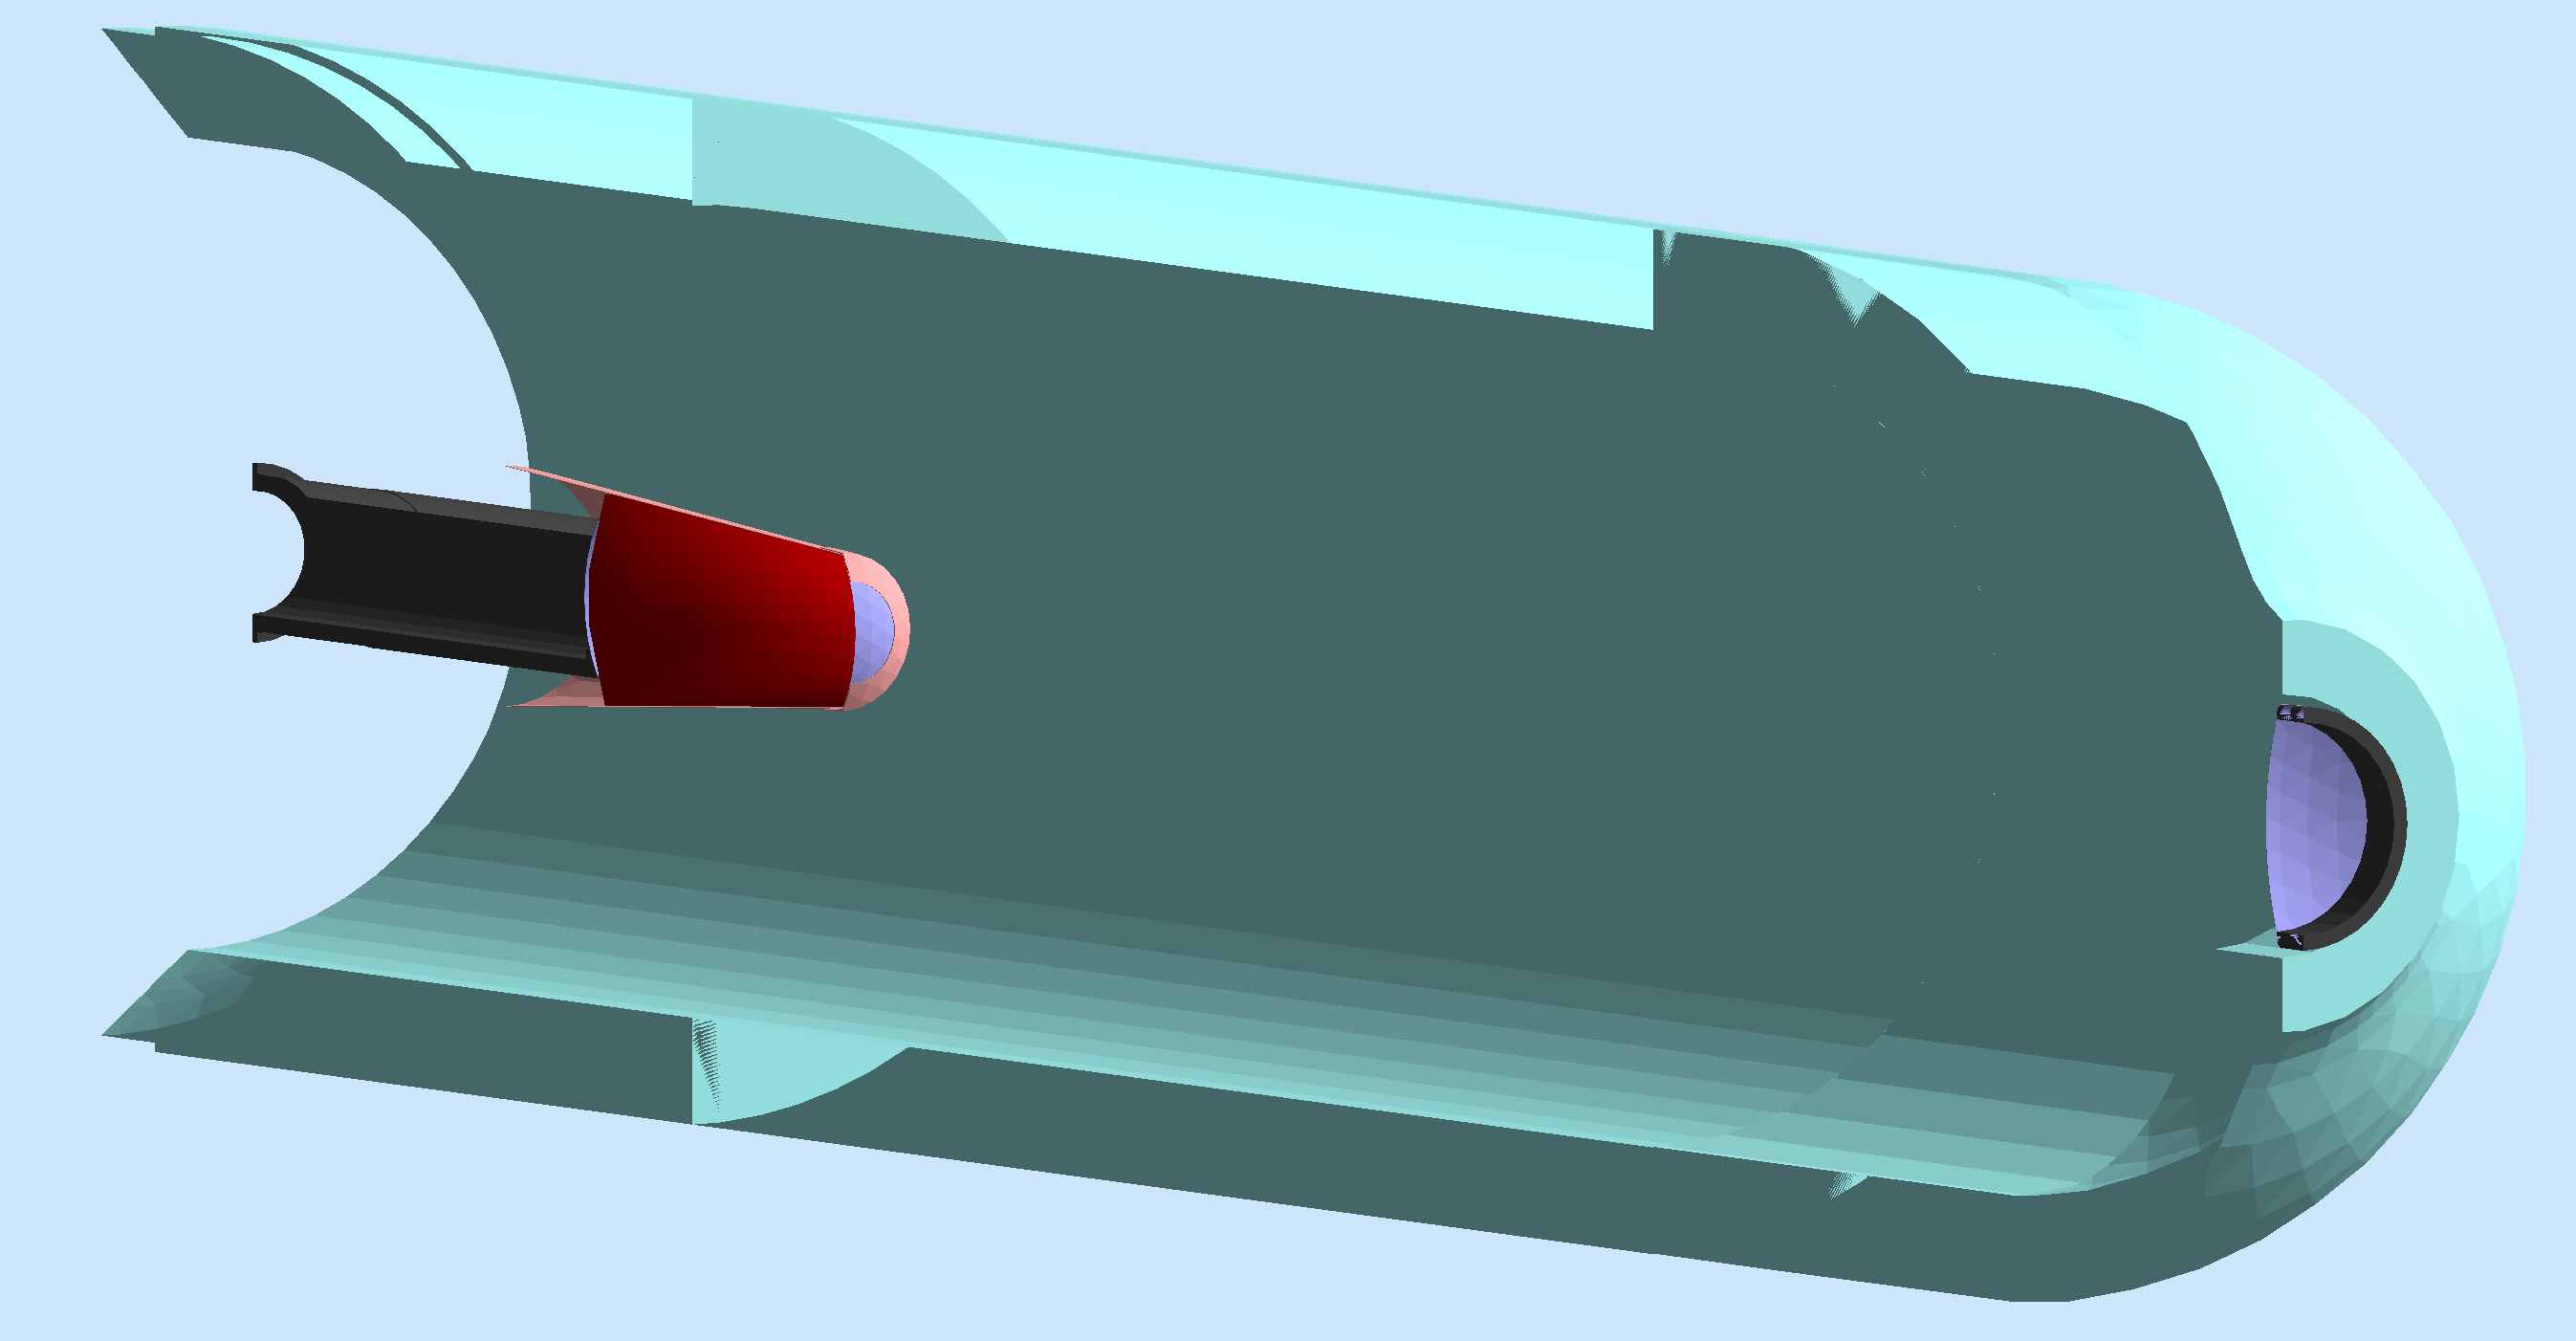
\includegraphics[width=0.95\columnwidth,keepaspectratio]{img/targetOverview1.png}
	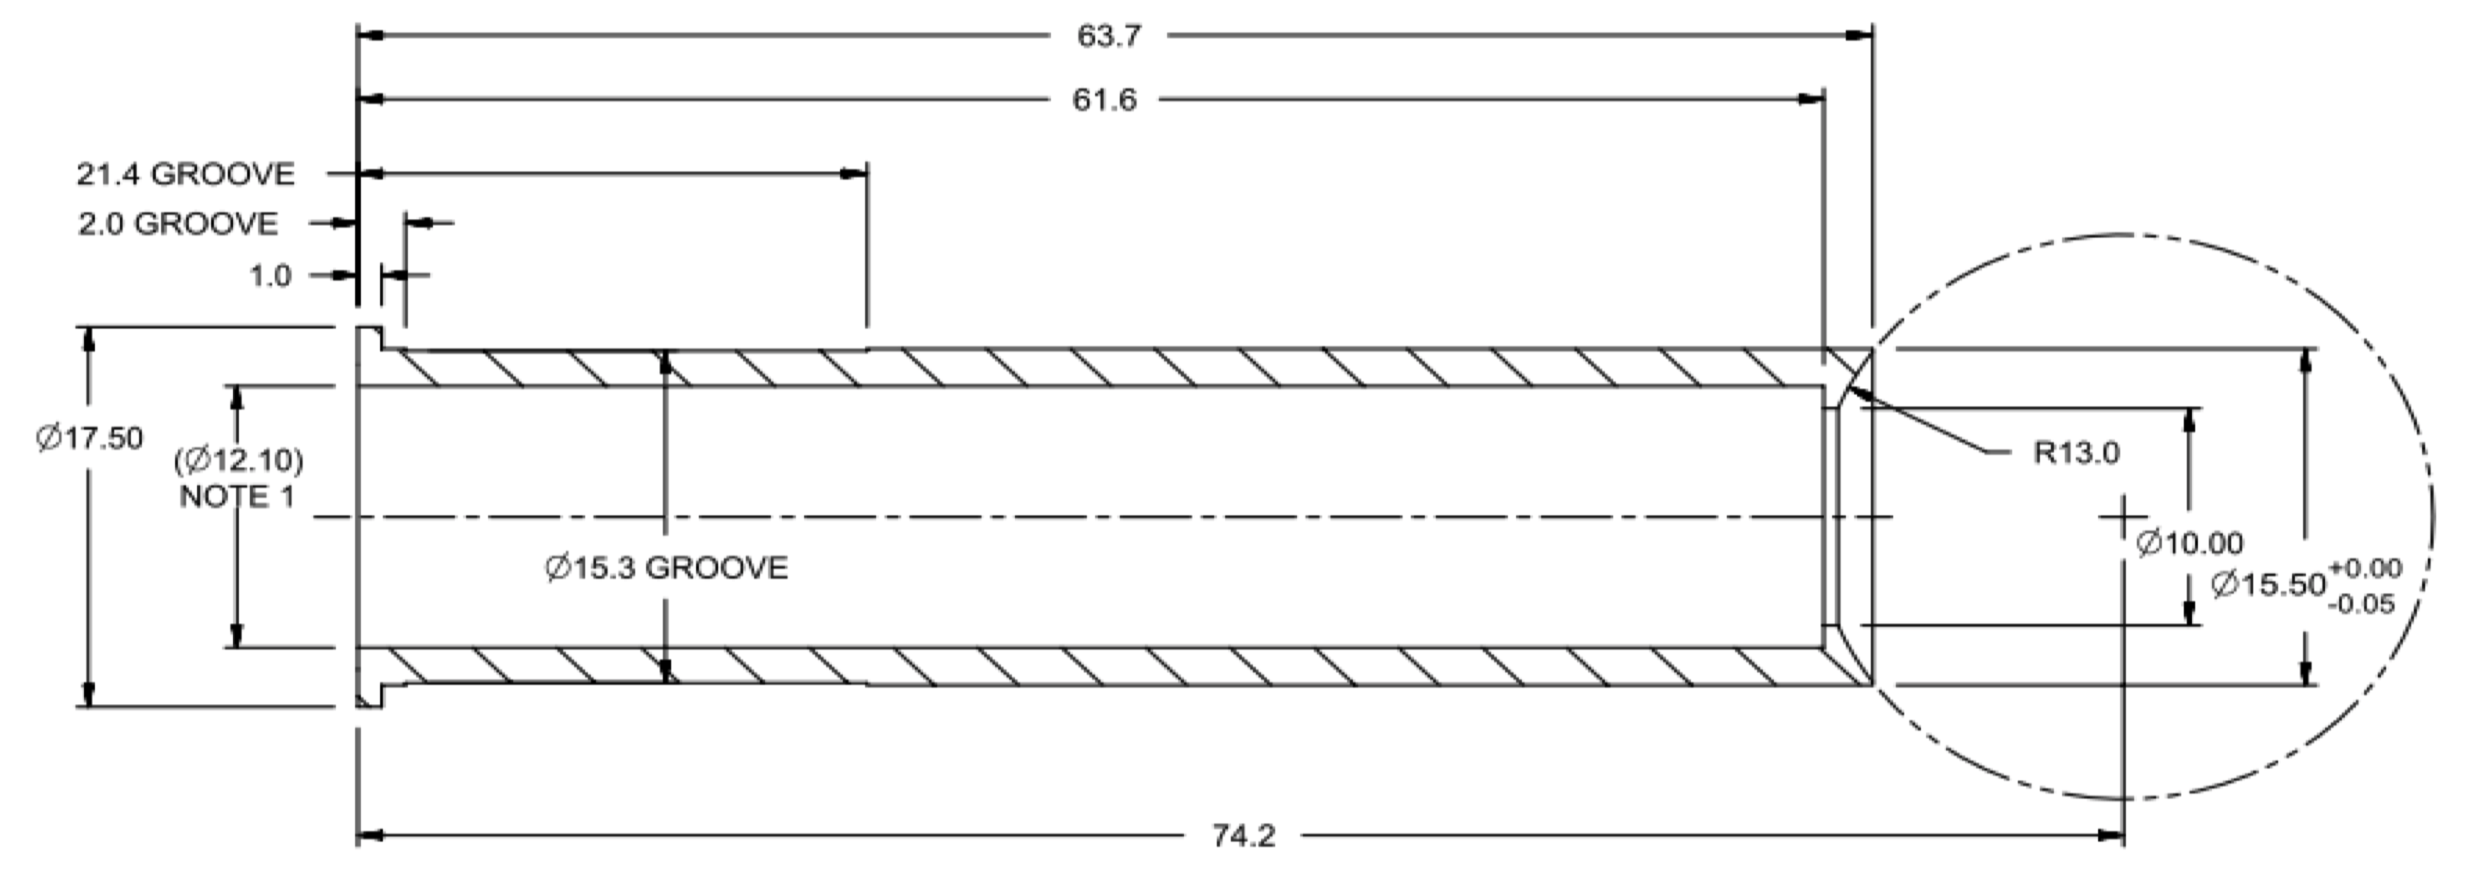
\includegraphics[width=0.95\columnwidth,keepaspectratio]{img/targetOverview2.png}
	\caption{Top: overview of the target implementation in GEMC includes the scattering chamber (cyan color), the
            downstream cup near the right of the figure and 50 μm aluminum window. Bottom: the torlon base
            tube starts at a radius of r=6.06 mm, and ends at r = 7.75 mm. It is 63.7 mm long.}
	\label{fig:targetDesign}
\end{figure}

\subsubsection{Geometry Git Location}
The github location of the gemc perl api scripts and the STL files is \url{https://github.com/gemc/detectors/tree/master/clas12/targets}.





